%%%% cs420.tex

\typeout{CS420 Course Project Report Template}

% This file is the template for CS420 course project report.
% It is based on the instructions for authors for IJCAI-19.

\documentclass{article}
\pdfpagewidth=8.5in
\pdfpageheight=11in
\usepackage{cs420}

% Use the postscript times font!
\usepackage{times}
\usepackage{soul}
\usepackage{url}
\usepackage[hidelinks]{hyperref}
\usepackage[utf8]{inputenc}
\usepackage[small]{caption}
\usepackage{graphicx}
\usepackage{amsmath}
\usepackage{booktabs}
\usepackage{algorithm}
\usepackage{algorithmic}
\urlstyle{same}

\title{Play Atari Games with Deep Reinforcement Learning}

\author{
    Zheng Yu
    \affiliations
    ACM Honors Class, Shanghai Jiao Tong University \emails
    dataisland@sjtu.edu.cn
}

\begin{document}

\maketitle

\begin{abstract}
  This report will introduce my experience of train Deep Reinforcement Learning Network. I mainly used two tricks to increase training speed and make agent perform better, one tricks is taking non-uniform random strategy in 
  $\epsilon$-greedy, and the other is using transfer learning way with dynamic learning way. I compare the results of the my improved method with the results of the ordinary method. My method can use less time to get better result in some games.
  
\end{abstract}

\section{Introduction}

In reality world we hope that artificial intelligence can make decisions for us,
such as autonomous driving. However there are not exact data can use for training in most cases,
we can only get the reward signal after an agent make its decision. So we create the reinforcement learning method, we can handle these reward signal by using reinforcement learning
way. And it also has a good deal with the lag of the reward signal

Playing Atari games is a good way to measure the quality of reinforcement learning algorithms.
I trained 5 Atari games using Double DQN and Dueling DQN, These five games environment are 
\begin{itemize}
    \item PongNoFrameskip-v4,
    \item FreewayNoFrameskip-v4,
    \item AtlantisNoFrameskip-v4,
    \item TutankhamNoFrameskip-v4,
    \item KrullNoFrameskip-v4.
\end{itemize}


\section{Deep Reinforcement Learning Method}

In this part, the Deep Reinforcement Learning method used in my project will be introduced, include Deep Q-learning(DQN) and its extensions.

\subsection{Deep Q-Learning}
DQN and Q-leanring are similar algorithms, they are both based on value iteration, but in ordinary Q-learning, when the state and action space are discrete and the dimension is not high, Q-Table can be used to store the Q value of each state action pair. 
When the state and action space are high-dimensional continuous, it is very difficult to use Q-table. 
So here we can transform the Q-table into a function fitting problem, by fitting a function  instead of Q-table to generate Q values. Therefore, we can think of the deep neural network has a good effect on the extraction of complex features, so we can combine Deep Learning and Reinforcement Learning become Deep Q-Learning.

\paragraph{Experience Replay Memory} Reinforcement learning agent stores the experiences consecutively in the buffer, so adjacent $(s,a,r,s′)$ transitions stored are highly likely to have correlation. To remove this, the agent samples experiences uniformly at random from the pool of stored samples $((s,a,r,s′) \sim U(D))$.

\paragraph{Target Network} DQN uses an iterative update that adjusts the action-values (Q) towards target values that are only periodically updated, thereby reducing correlations with the target; if not, it is easily divergy because the target continuously moves. The Q-learning update at iteration i uses the following loss function:
$$
L_i(\theta_i) = E[ ( r + \gamma \max_{a'} Q(s',a';\theta_i^-) - Q(s, a; \theta_i) )^2 ]
$$
in which $\gamma$ is the discount factor determining the agent’s horizon, $\theta_i$ are the parameters of the Q-network at iteration i and $\theta_i^-$ are the network parameters used to compute the target at iteration i. The target network parameters $\theta_i^-$ are only updated with the Q-network parameters ($\theta_i$) every $C$ steps and are held fixed between individual updates.

\subsection{Prioritized Experience Replay}
Experience playback allows online reinforcement learning agents to remember and reuse past experience. In past research, past experience (transition, a record in the experience pool, expressed in the form of primitive ancestors, including state, action, reward, discount factor, next state), only obtained by uniform sampling. However, this method, as long as you have had this experience, then it will be used again with the same probability as other experiences, ignoring the importance of each experience.
    As a proxy for learning potential, prioritized experience replay
    samples transitions with probability $p_t$
    relative to the last encountered absolute TD error:
$$
p_t \propto \left | R_{t+1}+\gamma_{t+1} \max_{\alpha'} q_{\theta}^-(S_{t+1},a')-q_\theta(S_t, A_t) \right|^\omega
$$

where $\omega$ is a hyper-parameter that determines the shape of
the distribution. New transitions are inserted into the replay
buffer with maximum priority, providing a bias towards recent transitions. This method is very sensitive to noise. This method often only replays a small part of the experience, and some TD-error large experience is replayed many times. It is easy to overfit. To overcome these difficulties, we randomized the priority.Prioritized replay changes the distribution of updates in an uncontrollable way. This changed the result.

\subsection{Double DQN}
Double DQN is the same as Nature DQN and has the same two Q-network structures. On the basis of Nature DQN, the problem of overestimation is eliminated by decoupling the selection of target Q-value actions and the calculation of target Q-value. 

In Double DQN, it is no longer to directly find the maximum Q value in each action in the target Q network, but to first find the action corresponding to the maximum Q value in the current Q network, namely
$$
a^{max}(S'_j, w) = \arg\max_{a'}Q(\phi(S'_j),a,w)
$$
Then use this selected action $a^{max}(S'_j, w)$ to calculate the target Q value in the target network. which is:
$$
y_j = R_j + \gamma Q'(\phi(S'_j),\arg\max_{a'}Q(\phi(S'_j),a,w),w')
$$
Except for the calculation method of the target Q value, the algorithm flow of the Double DQN algorithm and Nature DQN is the same.
\subsection{Dueling DQN}
Dueling DQN considers dividing the Q network into two parts. The first part is only related to the state $s$, and has nothing to do with the specific action $a$. This part is called the value function part, and it is written as $V(s)$, the second part is related to the state $s$ and action $a$. This part is called the Advantage Function part and is written as $A(s, a)$, 
\begin{figure}[H]
\centering
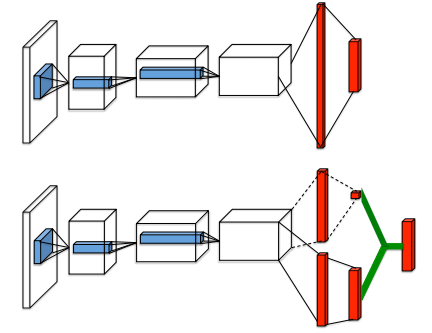
\includegraphics[width=0.4\textwidth]{img/dueling dqn.png}
\caption{Nature Network and Dueling Network}
\label{Fig.main2}
\end{figure}
Then in the end our value function can be re-expressed as:
$$
Q(s, a) = V(s) + A(s, a)
$$
the two network sharing a convolutional encoder, and merged by a special aggregator. This corresponds to
the following factorization of action values:
$$
Q(s,a) = V(S) + (A(s,a) - \frac{1}{|\mathcal{A}|}\sum\limits_{a' \in \mathcal{A}}A(S,a'))
$$
The structure can learn which state is valuable or worthless, rather than learning which action is valuable in this state. Because in some cases, we can choose any action in the current state, that is, the selected action has little effect on the environment.

\section{Optimize}
\subsection{Non-Uniform Random Strategy}
The optimization idea is based on enough knowledge of the game, so I will introduce and analyze the game itself in detail. 
\paragraph{Freeway}
The agent in this game needs to cross the freeway as much as possible within a limited time. The agent can choose to move forward, backward, or not move. If the agent encounters the car, it will move back a distance.

If I simply use uniform random strategy in Freeway game, the agent will move forward and backward with equal probability, and it will go backwards when it hits the car. So the probability of the agent reaching the end is very small and always just get zero reward signal. It leads much meaning less experience be put in replay buffer, 
thereby seriously reduces the learning efficiency. According to my experiment, I trained 1M frames
with Double DQN, but the agent still can not get any scores. This is obviously not conducive to exploration.

So I try to increase the probability of move forward from $\frac 1 3$ to $\frac 1 2$, the learning efficiency  be significantly improved. The agent can get 21 points after training just 10K frames. But I found that the agent just output 1 in fact, and this agent's performance has not increased anymore. That is not we want
to see. I think the reason is if the agent just simply move forward, it can get 21 scores! Hence the agent still not learn anything. Then I try to dynamically change the random action's distribution. I just try 
reduce the probability of move forward linearly from 0.8 to 0.3, it works good. Though the method the agent
can reach the baseline (30 scores) stably in 1.1M frames.

\paragraph{Atlantis}
In Atlantis games, there are three cannons on the base and plane fly in the air. The Agent's goal is to hit as many as planes to protect the Atlantis. Although the rewards obtained by the agent steadily increase with training, I still tried the same way in Freeway. 

I personally played this game and found that the agent cannot shoot continuously, or the cannons will do nothing. And if I only use the left
cannon and the middle cannon or only use right cannon, I can still get a high score. So I made a simple adjustment. In the first 1M frames, the $\epsilon$-greedy step will not choose to let the right cannons shoot, and ban the agent shoot continuously. After the 0.5M frames, the agent can get about 60K scores, but the baseline is 750K. Then I use common uniform random strategy, I totally trained 1.4M frames. The agent can get
at least 1M scores, much higher than baseline.

\subsection{Transfer Learning}
Not all games can use the above method, you need to have enough understanding of the game. 
When a game is more complicated, such as Krull and Tutankham, these two games involve more actions 
and more state. It is Difficult to find obvious features. So I have to think of other ways.

I observed the changes in the reward curve during training, I found two abnormal phenomena:
\begin{itemize}
    \item The reward suddenly increased to a high value, and then returned to a very low value and no longer increased for long times.
    \item Rewards are increasing steadily, but at a very slow rate, then suddenly dropped to a certain value. Then it started to rise slowly again.
\end{itemize}

For the first case, I tested the agent represented by the highest point in the reward curve. The agent can reach high level with low probability, or this agent is very unstable. I think the reason is the learning rate is too high resulting in a gradient explosion. If I change the learning rate to a smaller one and retrain the agent, it will waste much time. So at this time I thought of the transfer learning method. By this way I only need to continue the training process with low learning rate. After awhile, the agent will stop increasing again. This time is usually because
the exploration $\epsilon$ is too high, it leads most actions were acted by random. Replay buffer
 has no enough high score experience to learn. Because there is not universal descent method on
 exploration $\epsilon$ is considered good, I tuned it by myself with transfer learning method.
 
 The second case has the same problem, it is learning rate is too small. Then after a while the learning rate is too high, so the learning effect changes periodically.

\begin{figure}[H]
\centering
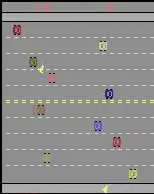
\includegraphics[width=0.2\textwidth]{img/Freeway.jpg}
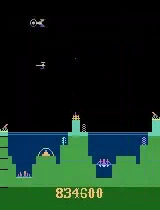
\includegraphics[width=0.193\textwidth]{img/Atlantis.jpg}
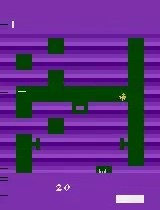
\includegraphics[width=0.2\textwidth]{img/Tu.jpg}
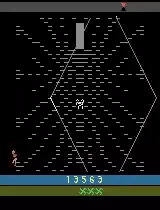
\includegraphics[width=0.2\textwidth]{img/Krull.jpg}
\caption{Atari games screenshot}
\label{Fig.main2}
\end{figure}

\section{Result}
This part will talk about the detail of out course project,
which includes the environment, and those result will
be shown in detail. The project has been put on github. (\href{https://github.com/cla7aye15I4nd/CloseAI}{CloseAI}).
\subsection{Environment}
PyTorch is the main tools in my project, 

\subsection{Performance}
This table is a comparison between my training results and previous training results
\begin{table}[H]
\centering
\begin{tabular}{llll}
\hline
Name  & DDQN & Prior.Duel. & \textit{My Idea} \\
\hline
Pong      & 19.1  & 18.4  & 20.0    \\
Freeway   & 28.8  & 28.2 &   30.5   \\
Atlantis  & 292,491.0  & 423,252.0   &  2,705,425.0 \\
Tutankham & 92.2  & 108.6 & 265.3 \\
Krull     & 7,658.6  & 7,658.6 & 11,135.0 \\
\hline
\end{tabular}
\caption{Training Result}
\label{tab:plain}
\end{table}

\subsection{Hyper Parameter}
Because of I used transfer learning, so the learning rate is not a constant. Only Pong just
 use single learning rate ($10^{-4}$), the Freeway and Krull has two stages, and Tutankham has
 three stages, Atlantis has four stages.
 
\begin{table}[H]
\centering
\begin{tabular}{ll}
\hline
Stage  & learning rate \\
\hline
1 & $1 \times 10^{-4}$\\
2 & $6.25 \times 10^{-5}$ \\
\hline
\end{tabular}
\caption{Freeway and Krull training learning rate}
\label{tab:plain}
\end{table}

\begin{table}[H]
\centering
\begin{tabular}{ll}
\hline
Stage  & learning rate \\
\hline
1 & $3.125 \times 10^{-4}$ \\
2 & $1 \times 10^{-4}$\\
3 & $6.25 \times 10^{-5}$ \\
4 & $1 \times 10^{-5}$ \\
\hline
\end{tabular}
\caption{Atlantis training learning rate}
\label{tab:plain}
\end{table}

\begin{table}[H]
\centering
\begin{tabular}{ll}
\hline
Stage  & learning rate \\
\hline
1 & $3.125 \times 10^{-4} $\\
2 & $10^{-4}$\\
3 & $6.25 \times 10^{-5}$ \\
\hline
\end{tabular}
\caption{Tutankham training learning rate}
\label{tab:plain}
\end{table}


\begin{table}[H]
\centering
\begin{tabular}{ll}
\hline
Parameter  & Value \\
\hline
Min history to start learning & 10K \\
Exploration $\epsilon$   & $1.0 \rightarrow 0.01$ \\
Target Network Period  & 10K \\
Prioritization exponent $\alpha$ & 0.6 \\
Prioritization importance sampling $\beta$    & $0.4 \rightarrow 1.0$ \\
Optimize interval & 4 \\
\hline
\end{tabular}
\caption{Training Hyper-parameter}
\label{tab:plain}
\end{table}

\begin{table}[H]
\centering
\begin{tabular}{ll}
\hline
Parameter  & Value \\
\hline
Q network: channels & 32, 64, 64 \\
Q network: filter size&  8 × 8, 4 × 4, 3 × 3\\
Q network: stride & 4, 2, 1\\
Q network: hidden units & 512\\
Q network: output units & Number of actions\\
Discount factor $\gamma$ & 0.99\\
Memory size & 50K transitions\\
Minibatch size & 32 \\
\hline
\end{tabular}
\caption{Network Hyper-parameter}
\label{tab:plain}
\end{table}

\section{Conclusion}
Most deep reinforcement learning paper use only a single learning rate, but it is not always a good way. Because the learning speed of the agent is unpredictable. If we want to spend less time on training, multi-stage training will be a better idea. 

Although my training results are numerically excellent, the agent behaves in a way that is not what we want. For example, the behavior pattern of the agent is the same every round when play pong.

\begin{figure}[H]
\centering

\includegraphics[width=0.15\textwidth]{img/frame_007_delay-0.1s.jpg}

\includegraphics[width=0.15\textwidth]{img/frame_015_delay-0.1s.jpg}
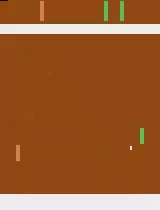
\includegraphics[width=0.15\textwidth]{img/frame_017_delay-0.1s.jpg}
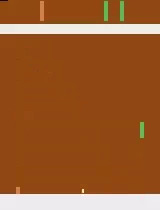
\includegraphics[width=0.15\textwidth]{img/frame_019_delay-0.1s.jpg}
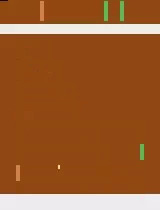
\includegraphics[width=0.15\textwidth]{img/frame_020_delay-0.1s.jpg}

\includegraphics[width=0.15\textwidth]{img/frame_022_delay-0.1s.jpg}
\caption{Pong screenshot}
\label{Fig.main2}
\end{figure}

After finish the Deep Reinforcement Learning project, I learned much reinforcement 
learning methods. Although some method I have no time to implement, These knowledge and ideas will still play a role in my future study and research. The following are some lessons I learned from this project:

\begin{itemize}
    \item Thick twice, code once.
    \item Don’t just trust paper but own judgment.
    \item Stay patient and calm when fail.
    \item Sometimes lucky is important.
\end{itemize}

\appendix

\nocite{2015arXiv151106581W}
\nocite{2017arXiv171002298H}
\nocite{2015arXiv150906461V}
\nocite{2013arXiv1312.5602M}
\nocite{2015arXiv151105952S}
\nocite{2017arXiv170706887B}
\nocite{2015Natur.518..529M}
\nocite{2016arXiv160602228M}
\nocite{2015arXiv150201852H}

\bibliographystyle{named}
\bibliography{cs420}

\end{document}

